\section{Preliminary Building Blocks}

\subsection{Recurrent Neural Networks (RNN)}

\subsubsection{Motivation for RNNs}

Traditional neural networks cannot persist information. As a comparison, while humans do not start thinking from scratch each time they learn something new, neural networks lack memory. Inherently related to sequences, recurrent neural networks use a recurrence or looping mechanism to introduce data persistence in the model to overcome this problem (Colah, 2015). This looping mechanism acts like a ``highway" to flow from one step to the next by passing inputs and modified hidden states along until computing a final prediction (Nguyen, 2018a). 

\begin{figure}[h]
\centering
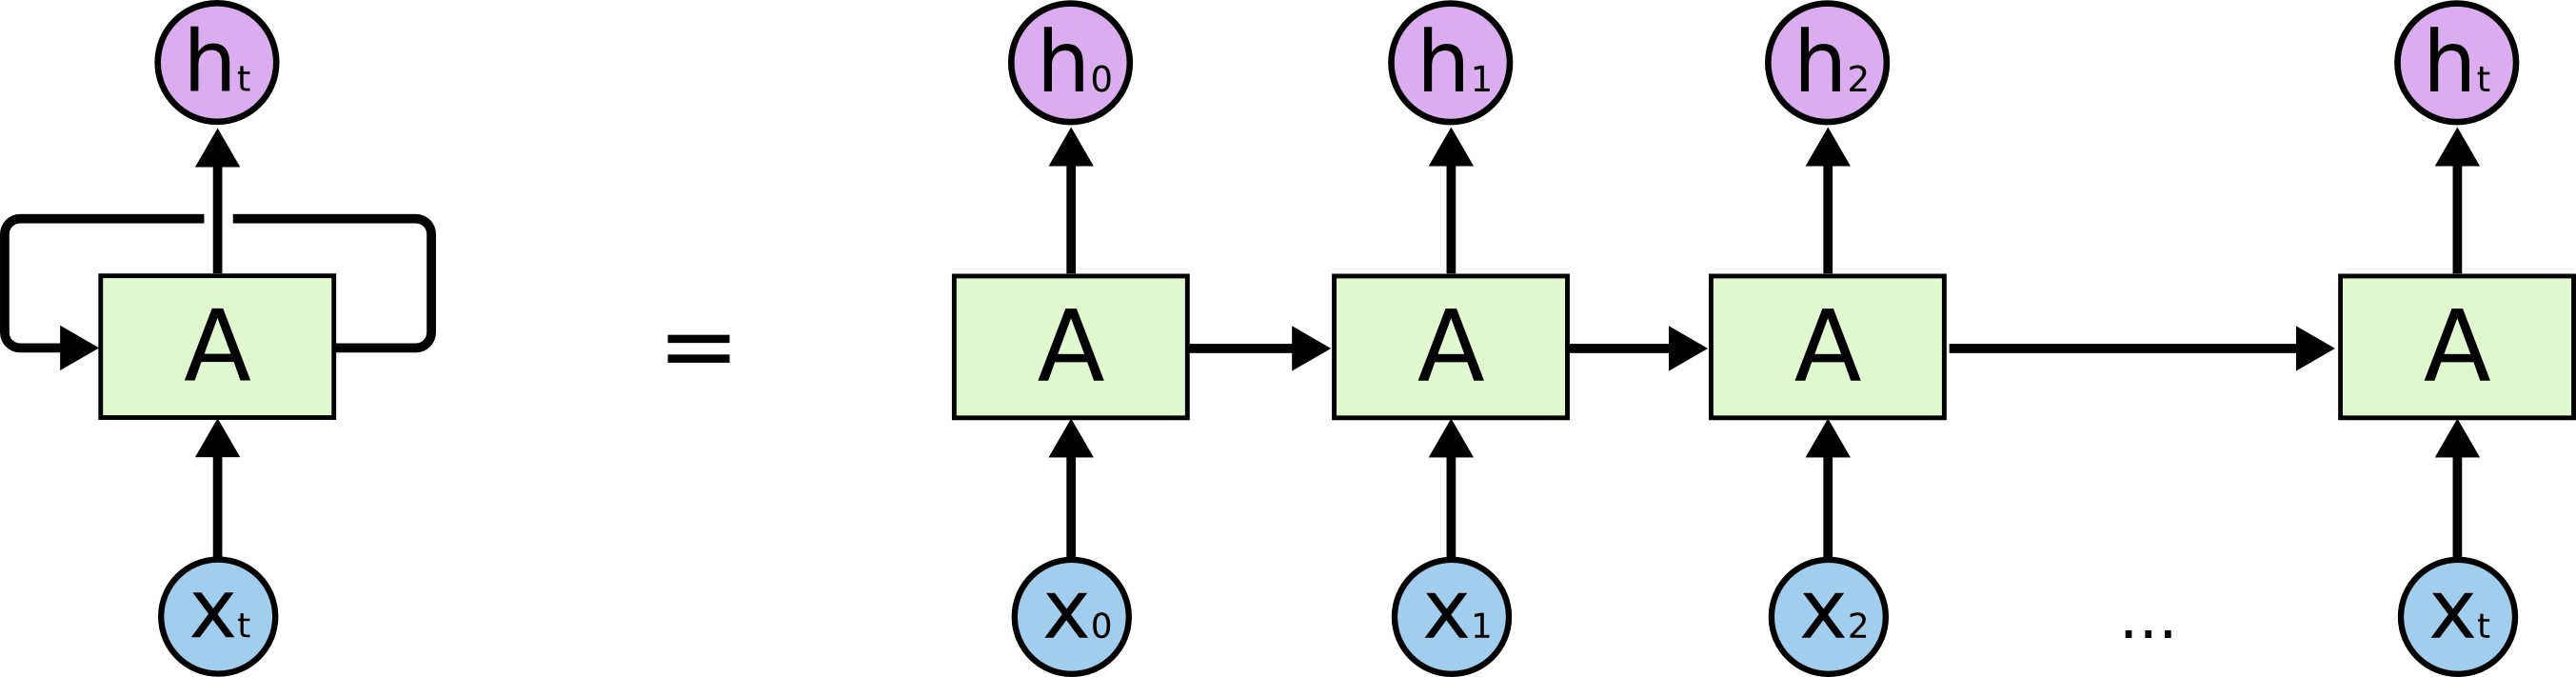
\includegraphics[width=0.7\textwidth]{imgs/rnn_colah_unrolled.png}
\caption{Unrolled view of Recurrent Neural Network with Hidden States $h_i$ and inputs $x_i$. From \emph{Understanding LSTMs}, by Colah., 2015. \url{https://colah.github.io/posts/2015-08-Understanding-LSTMs/}. Copyright 2015 by Colah.}
\end{figure}


\subsubsection{Describing RNNs}

An RNN is a unidirectional language model in that it uses infinite \emph{left} context words to the left of the target word. It is a neural network consisting of a hidden state vector $\overrightarrow{h}$ and output vector $\overrightarrow{y}$ and takes a sequence (sentence) of input symbols (words) $\overrightarrow{x} = \{ x_1, ..., x_T\}$, where each $x_i$ is a word. At each time step $t$ the current hidden state $h_t$ is updated via the formula $h_t = f \Big( h_{t-1}, x_t \Big)$ where $f(\cdot)$ is a nonlinear activation function. The RNN's intermediate task is to predict a probability distribution over an input sequence (sentence) by predicting the next word symbol $x_t$ in the sequence sentence, using left context, so the output at time $t$ is the conditional distribution $P \Big(x_t \; | \; x_{t-1}, ..., x_1 \Big)$. The probability of the entire sequence sentence $\overrightarrow{x}$ is the product of all the probabilities of the individual words, $P(\overrightarrow{x}) = \prod_{t=1}^T P \Big(x_t \; | \; x_{t-1}, ..., x_1 \Big)$ (Cho, 2014). 

Nguyen (2018b) describes the basic workflow of RNNs as follows: 

\begin{enumerate}
    \item First, words are transformed into numeric vectors, allowing the RNN to process the vector sequence, taking one vector at a time. 
    
    \begin{figure}[h]
    \centering
    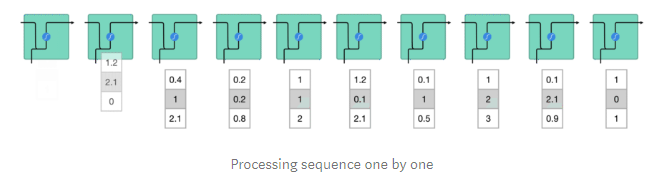
\includegraphics[width=0.8\textwidth]{imgs/rnn_step1.png}
    \caption{RNN Processing Inputs One at a Time. From \emph{Illustrated Guide to Recurrent Neural Networks}, by Nguyen, 2018.\url{https://towardsdatascience.com/illustrated-guide-to-lstms-and-gru-s-a-step-by-step-explanation-44e9eb85bf21}. Copyright 2018 by Nguyen.}
    \end{figure}
    
    \item While processing the inputs in the above step, the RNN passes previous hidden state to the next step of the sequence. The hidden state serves as memory for the network by holding previous information. 
    
    To calculate hidden state for a particular cell in the RNN, the input and previous hidden state are combined to form a vector, which is then passed through a $\text{"tanh"}$ activation function so that its components are squashed betwen $-1$ and $1$ to avoid large values. The output of this operation becomes the new hidden state. 
    
    \begin{figure}[h]
    \centering
    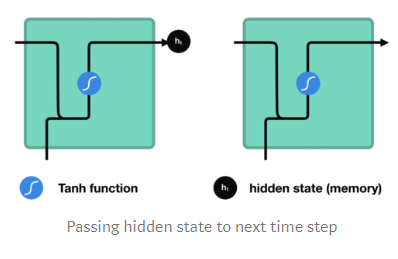
\includegraphics[width=0.4\textwidth]{imgs/rnn_step2.png}
    \caption{Hidden State Goes Through Tanh Activation. From \emph{Illustrated Guide to Recurrent Neural Networks}, by Nguyen, 2018. \url{https://towardsdatascience.com/illustrated-guide-to-lstms-and-gru-s-a-step-by-step-explanation-44e9eb85bf21}. Copyright 2018 by Nguyen.}
    \end{figure}
    
    \item This process is repeated until an output prediction word is generated. 
    
\end{enumerate}


    
\subsection{Long-Short Term Memory Networks (LSTM)}

\subsubsection{Motivation for LSTM: Problem with RNNs}

RNNs suffer from the well known \textbf{long-term dependency problem}. In some prediction tasks, longer context is needed to predict a target word. For instance to predict the last word in the sentence ``I grew up in France ... I speak fluent \emph{French}", a model would need the earlier context word ``France." When this gap between target and context words becomes too large, RNNs cannot learn their relationship, thus showing its lack of handling \textbf{long-term dependencies} (Colah, 2015). 

\begin{figure}[h]
\centering
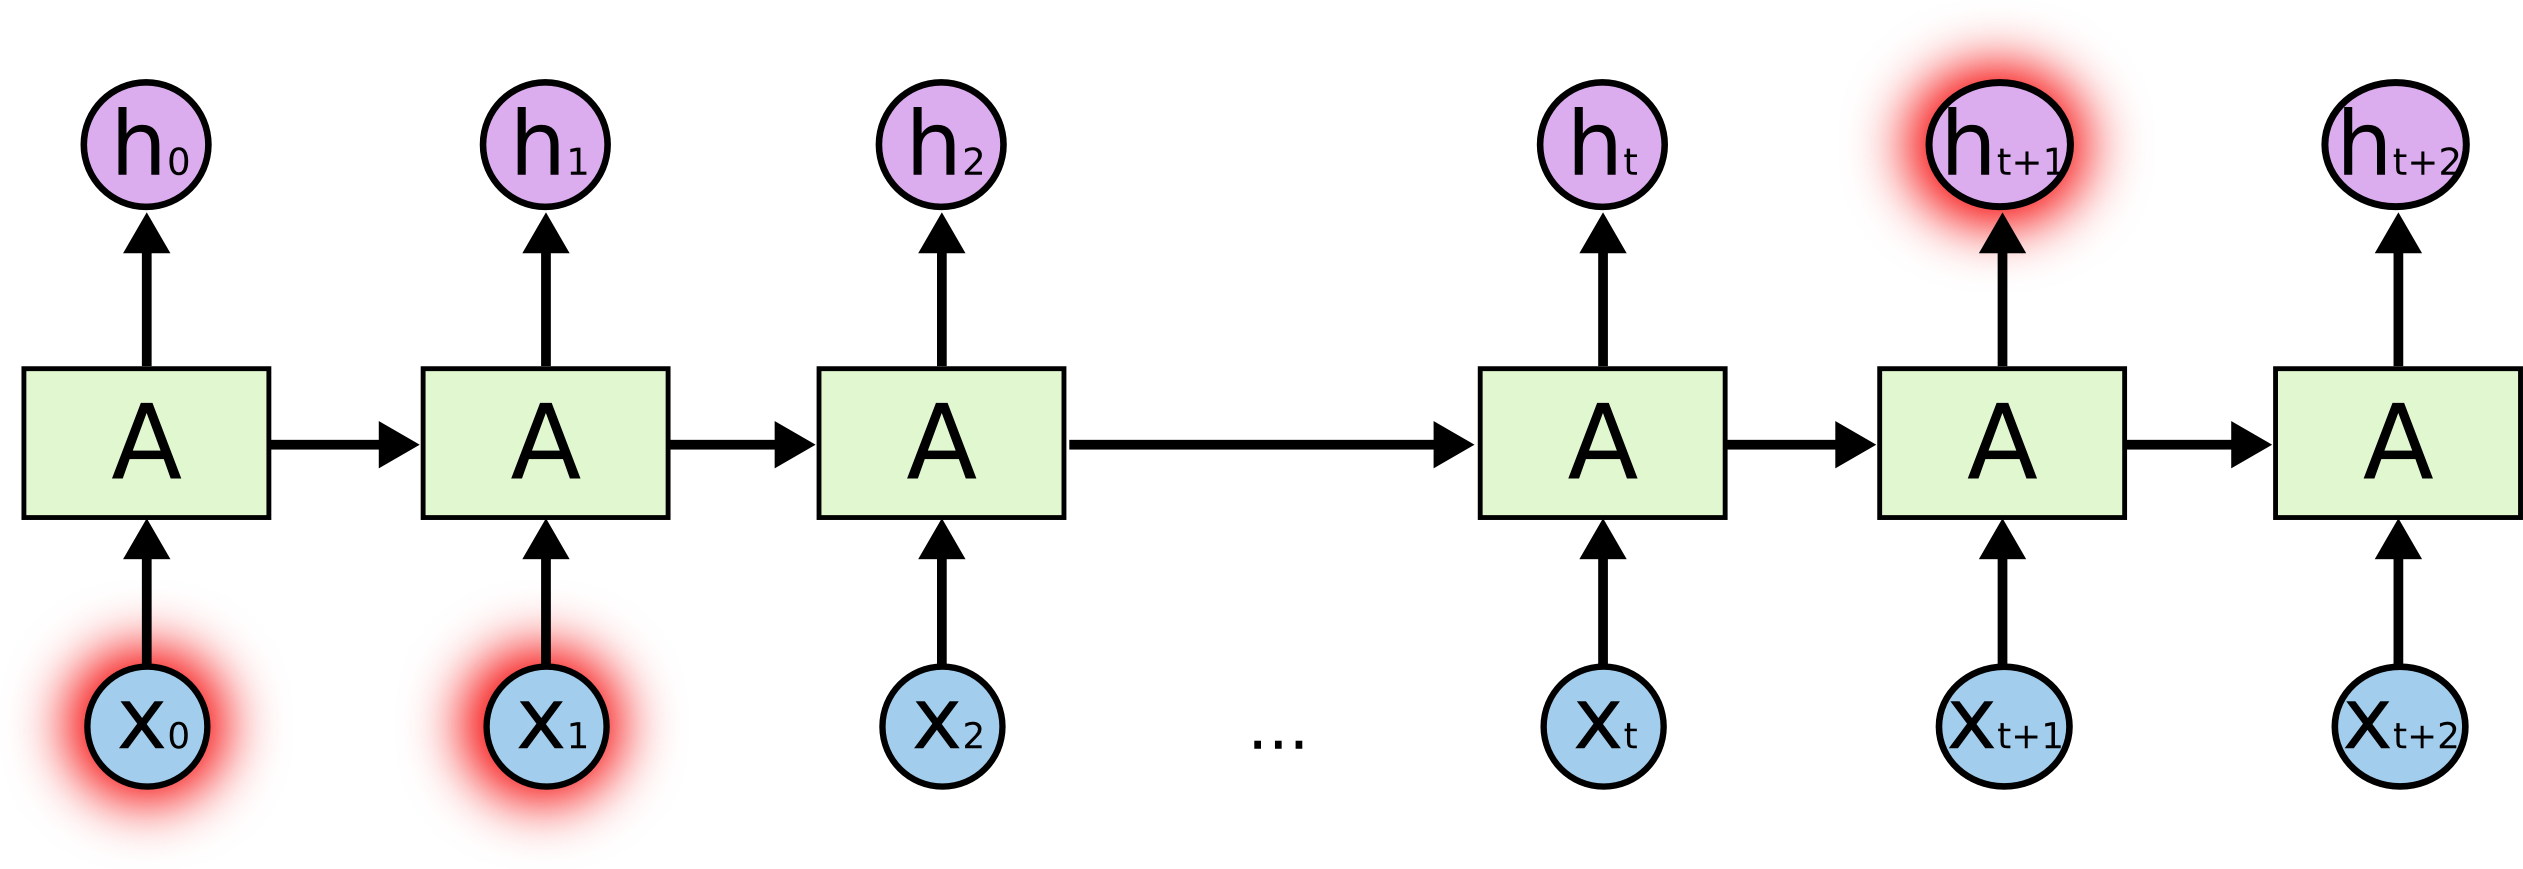
\includegraphics[width=0.6\textwidth]{imgs/rnn_longterm.png}
\caption{Long-Term Dependency Problem in RNNs (widening gap between inputs $x_i$ and hidden states $h_j$. From \emph{Understanding LSTMs}, by Colah, 2015. \url{https://colah.github.io/posts/2015-08-Understanding-LSTMs/}. Copyright 2015 by Colah.}
\end{figure}

The \textbf{short-term memory problem} occurs due to the \textbf{vanishing gradient problem}. During backward propagation of errors through the neural network (described in Appendix A), the gradient shrinks as it back propagates through time and becomes too small to update the parameter weights significantly. This is compounded by the fact that since inputs at any timestep $t$ are dependent on previous $t-1$ outputs, longer sequences require more gradient calculations. Adjustments to earlier layers thus become smaller, causing gradients to shrink exponentially as they are backpropagated through to earlier layers of the RNN. As a result, RNNs ``forget" older history, resulting in short-term memory (Nguyen, 2018b). 


\subsubsection{Describing LSTMs}
A long-short term memory network (LSTM) is a type of RNN that sequentially extracts information from each word in a sentence and embeds the information into a semantic vector. 

Long-short term memory networks (LSTM) learn long-term information by design, contrary to RNNs. LSTMs use features such as \textbf{cell state} and \textbf{gates} to regulate information flow from earlier time steps to later time steps. The gates are separate neural networks that decide which information to add or remove from the cell state, thus explicitly letting the LSTM ``remember" or ``forget" information (Nguyen, 2018b). Simply, LSTMs differ from RNNs in their repeating module since the standard RNN contains a single $\text{tanh}$ activation layer while the LSTM contains the four neural network layers (gates). This difference is illustrated in Figure 11.


\begin{figure}[h]
\centering
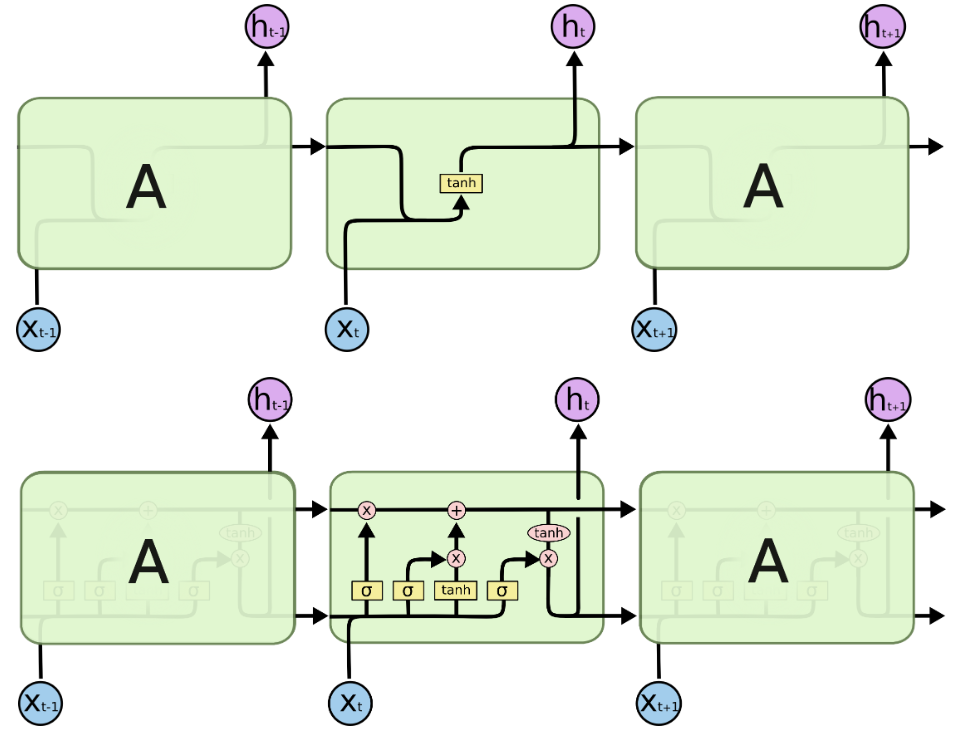
\includegraphics[width=0.7\textwidth]{imgs/rnn_vs_lstm_cells.png}
\caption{RNN's (top figure) repeating module has a single layer while LSTM's (bottom figure) repeating module has several interaction layers or gates. Yellow box denotes a \emph{neural network layer}; pink circle denotes \emph{pointwise operation} between vectors; single arrow denotes \emph{vector transfer}; two converging arrows mean \emph{concatenation operation}, and two diverging arrows mean \emph{copy operation}. From \emph{Understanding LSTMs}, by Colah, 2015. \url{https://colah.github.io/posts/2015-08-Understanding-LSTMs/}. Copyright 2015 by Colah.}
\end{figure}

Since LSTMs can accumulate increasingly richer information while parsing the sentence, by the time the last word is reached, the hidden layer of the network provides a \textbf{semantic representation} of the entire sentence (Palangi et al., 2016). 

A core idea in an LSTM is the \textbf{cell state}, which is shown in Figure 11 as the topmost line with the gates merging into it. For example, for a language predicting the next word based on previous ones, the cell state might include the gender of the present subject so that the correct pronouns are used. When a new subject is observed, the cell state should forget the old subject's gender and retain the new one (Colah, 2015). 

From Nguyen (2018b), the gates (neural network layers) regulating information are as follows: 

\begin{itemize}
    \item \textbf{Forget Gate: } the forget gate decides information to discard or keep. The previous hidden state $h_{t-1}$ and current input $x_t$ are passed through the sigmoid nonlinearity function. The forget gate outputs a number between $0$ and $1$ for each number in the cell state $C_{t-1}$; values closer to $0$ indicate the forget gate should discard the information and values closer to $1$ should be kept. 
    $$
    f_t = \sigma \Big( W_f \cdot [h_{t-1}, x_t] + b_f \Big)
    $$
    where $f_t$ denotes the forget gate for time $t$, $\sigma(\cdot)$ denotes the sigmoid, $W_f$ denotes the weight matrix at the forget layer, and $b_f$ denotes the forget gate's bias term. 
    
    \item \textbf{Input Gate: } the input gate $i_t$ updates the cell state $C_t$, similarly to the forget gate. Previous hidden state $h_{t-1}$ and current input $x_t$ are passed though a signmoid function which decides values to update by normalizing vector cells to be between $0$ and $1$. The input gate is later used with the cell state to decide how values are updated. 
    $$
    i_t = \sigma \Big( W_i \cdot [h_{t-1}, x_t] + b_i \Big)
    $$
    where $i_t$ denotes the input gate for time $t$, $\sigma(\cdot)$ denotes the sigmoid, $W_i$ denotes the weight matrix at the input layer, and $b_i$ denotes the input gate's bias term. 
    
    \item \textbf{Cell State: } Current cell state $C_t$ is calculated similarly by taking in $h_{t-1}$ and $x_t$ and normalizing this to be between $-1$ and $1$ via a hyperbolic tangent nonlinearity:
    $$
    C_t = \tanh \Big( W_C \cdot [h_{t-1}, x_t] + b_C \Big)
    $$
    where $C_t$ denotes the cell state for time $t$, $\tanh(\cdot)$ denotes the hyperbolic tangent, $W_C$ denotes the weight matrix at the cell state layer, and $b_C$ denotes the cell state's bias term. 
    Next, the current cell state $C_t$ is pointwise multiplied by the input gate vector $i_t$ and the previous cell state $C_{t-1}$ is pointwise  multiplied by the forget gate vector $f_t$. The results are added to decide how information is remembered in the LSTM:
    $$
    C_t = f_t \cdot C_{t-1} + i_t \cdot C_t
    $$
    
    \item \textbf{Output Gate: }the output gate determines the next hidden state by multiplying the previous output state by the cell state that is filtered by the hyperbolic tangent. 
    $$
    o_t = \sigma \Big( W_o \cdot [h_{t-1}, x_t] + b_o \Big) \\
    h_t = o_t \cdot \tanh(C_t)
    $$
    
\end{itemize}



\begin{SCfigure}
  \centering
  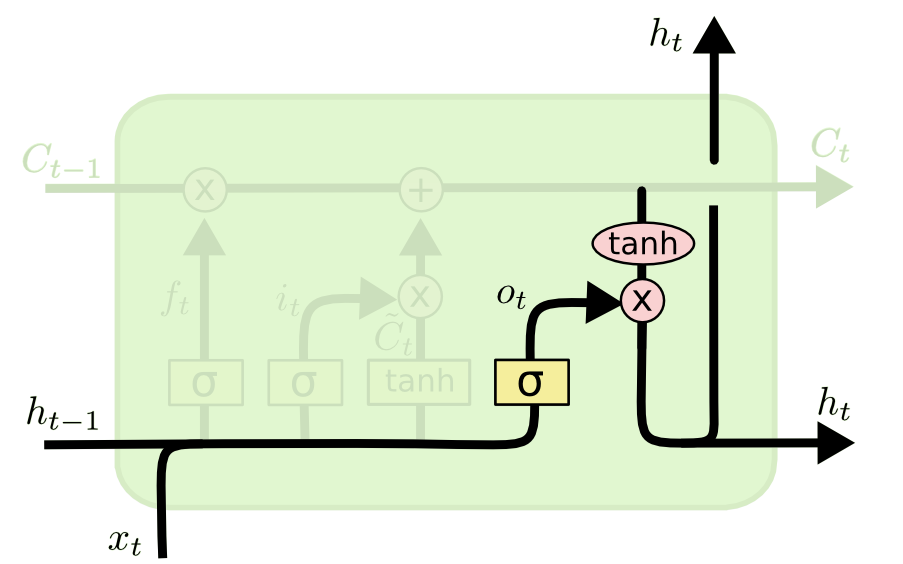
\includegraphics[width=0.8\textwidth]{lstm_outputGate.png} 
  \caption{\textbf{Output Gate Calculation: } 
  $$\begin{array}{ll}
    o_t = \sigma \Big( W_o \cdot [h_{t-1}, x_t] + b_o \Big) \\
    h_t = o_t \cdot \tanh(C_t)
  \end{array}$$}
\end{SCfigure}
    

\subsection{Gated Recurrent Networks (GRU)}

\subsection{Convolutional Neural Networks (CNN)}